
%(BEGIN_QUESTION)
% Copyright 2010, Tony R. Kuphaldt, released under the Creative Commons Attribution License (v 1.0)
% This means you may do almost anything with this work of mine, so long as you give me proper credit

Calculate the voltage across the bridge ($V_{AB}$) at the following RTD temperatures, assuming a 604 $\Omega$ nickel-iron RTD with an alpha value of 0.00518:

$$\includegraphics[width=15.5cm]{i00600x01.eps}$$

\begin{itemize}
\item{} $T$ = 0 $^{o}$C ; $V_{AB}$ = \underbar{\hskip 50pt} millivolts
\vskip 10pt
\item{} $T$ = 81 $^{o}$C ; $V_{AB}$ = \underbar{\hskip 50pt} millivolts 
\vskip 10pt
\item{} $T$ = -45 $^{o}$C ; $V_{AB}$ = \underbar{\hskip 50pt} millivolts 
\vskip 10pt
\item{} $T$ = 320 $^{o}$F ; $V_{AB}$ = \underbar{\hskip 50pt} millivolts 
\end{itemize}


\underbar{file i00600}
%(END_QUESTION)





%(BEGIN_ANSWER)

All answers shown here based on tabulated values for the RTD's resistance (rather than values calculated by formula):

\begin{itemize}
\item{} $T$ = 0 $^{o}$C ; $V_{AB}$ = {\bf -0.6989} millivolts
\vskip 10pt
\item{} $T$ = 81 $^{o}$C ; $V_{AB}$ = {\bf 0.9568} millivolts 
\vskip 10pt
\item{} $T$ = -45 $^{o}$C ; $V_{AB}$ = {\bf -1.6215} millivolts 
\vskip 10pt
\item{} $T$ = 320 $^{o}$F ; $V_{AB}$ = {\bf 2.4831} millivolts 
\end{itemize}


%(END_ANSWER)





%(BEGIN_NOTES)


%INDEX% Measurement, temperature: RTD (bridge circuit)

%(END_NOTES)

